% !TeX encoding = UTF-8
% !TeX program = xelatex
% !TeX spellcheck = en_US

\documentclass{YNUbachelor}
\usepackage{myPackages}

\title{云南大学本科学生毕业论文(设计)\;\LaTeX 模板}
\school{XX学院}
\author{XXX}
\studentID{20181050000}
\major{XX学}
\teacher{XXX}

\begin{document}
	
	\cover

	\copyrightpage
	
	\maketitle

	\toc

	\begin{abstract}
		中文摘要
	\end{abstract}

	\keywords{关键词1;关键词2;关键词3}

	\begin{enabstract}
		英文摘要
	\end{enabstract}

	\enkeywords{enKeyWords1;enKeyWords2;enKeyWords3}
		
	\section{绪论}
		{\bfseries \songti 宋体加粗}
		
		{\bfseries \heiti 黑体加粗}
		
		内容内容内容内容内容内容内容内容内容内容内容内容内容内容内容内容内容内容内容内容内容内容内容内容内容内容内容内容内容内容内容内容内容内容内容内容内容内容内容内容内容内容内容内容内容内容内容内容内容内容内容内容内容内。容内容内容内容内容内容内容内容内容内容内容内容内容内容内容内容内容内容内容内容内容内容内容内容内容内容内容内容内容内容内容内容内容内容内容内容内容。
		
	\subsection{介绍}
		内容内容内容内容内容内容内容内容内容内容内容内容内容内容内容内容内容内容内容内容内容内容内容内容内容内容内容内容内容内容内容内容内容内容内容内容内容内容内容内容内容内容内容内容内容内容内容内容内容内容内容内容内容内。容内容内容内容内容内容内容内容内容内容内容内容内容内容内容内容内容内容内容内容内容内容内容内容内容内容内容内容内容内容内容内容内容内容内容内容内容。
		
	\subsubsection{图表}
		内容内容内容内容内容内容内容内容内容内容内容内容内容内容内容内容内容内容内容内容内容内
		
		\lstinputlisting[language=Python,float=htbp]{code/Python example.py}
		
		容内容内容内容内容内容内容内容内容内容内容内容内容内容内容内容内容内容内容内容内容内容内容内容内容内容内容内容内容内容内容内容内。容内容内容内容内容内容内容内容内容内容内容内容内容内容内容内容内容内容内容内容内容内容内容内容内容内容内容内容内容内容内容内容内容内容内容内容内容。
	
	\begin{figure}[htbp]
		\centering
		\includegraphics[width=0.7\linewidth]{fig}
		\caption{这是一个示例图片}
		\label{fig:fig}
	\end{figure}

	内容内容内容,引用图片\autoref{fig:fig}内容内容内容
	\begin{verbatim}
		\begin{figure}[htbp]
			\centering
			\includegraphics[width=0.7\linewidth]{figures/fig.jpg}
			\caption{这是一个示例图片}
			\label{fig:fig}
		\end{figure}
	\end{verbatim}
	

	内容内容内容内容内容内容内容内容内容内容内容内容内容内容内容内容内容内容内容内容内容内容内容内容内容内容内容内容内容内容内容内容内容内容内容内容内容内容内容内容内容内容内容内容内容内容内容内容内容内容内容内容内容内。容内容内容内容内容内容内容内容内容内容内容内容内容内容内容内容内容内容内容内容内容内容内容内容内容内容内容内容内容内容内容内容内容内容内容内容内容内容内容。
	
	\begin{table}[htbp]
		\centering
		\caption{An example table.}
		\label{tab:example}
		\begin{tabular}{lcc}
			\toprule
			Star & Mass & Luminosity\\
			& $M_{\odot}$ & $L_{\odot}$\\
			\midrule
			Sun & 1.00 & 1.00\\
			$\alpha$~Cen~A & 1.10 & 1.52\\
			$\epsilon$~Eri & 0.82 & 0.34\\
			\bottomrule
		\end{tabular}
	\end{table}
	\autoref{tab:example} 由如下代码生成:
	\begin{verbatim}
		\begin{table}[htbp]
			\centering
			\caption{An example table.}
			\label{tab:example}
			\begin{tabular}{lcc}
				\toprule
				Star & Mass & Luminosity\\
				& $M_{\odot}$ & $L_{\odot}$\\
				\midrule
				Sun & 1.00 & 1.00\\
				$\alpha$~Cen~A & 1.10 & 1.52\\
				$\epsilon$~Eri & 0.82 & 0.34\\
				\bottomrule
			\end{tabular}
		\end{table}
	\end{verbatim}

	\subsubsection{公式}
	
	勾股定理
	\begin{align}
		a^2+b^2=c^2\label{eq:0}
	\end{align}
	\autoref{eq:0}代码如下:
	\begin{verbatim}
		\begin{align}
			a^2+b^2=c^2\label{eq:0}
		\end{align}
	\end{verbatim}
	
	\section{结论}
	引用\cite{向守平2008天体物理概论}。引用\cite{BQC_2020}。
	\begin{acknowledgement}
		致谢。
	\end{acknowledgement}

	\begin{reference}%参考文献
		\bibliography{references/references.bib}%.bib文件路径, 文献的bibtex格式信息
	\end{reference}
	
	\backcover%封底
\end{document}
